\documentclass{article}

% if you need to pass options to natbib, use, e.g.:
% \PassOptionsToPackage{numbers, compress}{natbib}
% before loading nips_2017
%
% to avoid loading the natbib package, add option nonatbib:
% \usepackage[nonatbib]{nips_2017}

\usepackage[final]{nips_2017}


\usepackage[utf8]{inputenc} % allow utf-8 input
\usepackage[T1]{fontenc}    % use 8-bit T1 fonts
\usepackage{hyperref}       % hyperlinks
\usepackage{url}            % simple URL typesetting
\usepackage{booktabs}       % professional-quality tables
\usepackage{amsfonts}       % blackboard math symbols
\usepackage{nicefrac}       % compact symbols for 1/2, etc.
\usepackage{microtype}      % microtypography
\usepackage{graphicx}


% Choose a title for your submission
\title{Tackling Story Cloze Test with Wrong Ending Generation}


\author{Pascal Wiesmann \qquad Stefano Woerner \qquad Sandar Felicity Lim}
%\graphicspath{{fig/}}
\begin{document}
% \nipsfinalcopy is no longer used

\maketitle

% We do not requrire you to write an abstract. Still, if you feel like it, please do so.
%\begin{abstract}
%\end{abstract}

\section{Introduction}

The training set of the story cloze test comes with only positive sample (i.e. stories with correct endings). On the other hand, the test set requires a classification as correct/wrong endings. This is one of the main difficulties with the story cloze test. We decided to generate wrong endings and to train a RNN-based classifier, using the correct endings from the training set and our own generated wrong endings. We explore several methods for the generation of wrong endings, which we will explain in section 2.

\section{Methodology}

\subsection{Model: Classifier}

Figure \ref{Figure:model} shows the architecture of our model. This is similar to the approach by Burgert et al. except for a few differences \cite{top4}. Our model involves two Long Short-Term Memory (LSTM) units to compute the feature representation of each sentence \citep{lstm}, instead of a Bidirectional Recurrent Neural Network (BiLSTM). We also use the last output of the LSTM instead of the last cell state.

Firstly, we looked up the word embedding of each word in vector space for each sentence. The embeddings from the first four sentences were then passed on to the first LSTM which summarises the story in numbers. Likewise, the last sentence was passed on to the second LSTM. The results of two LSTMs are then concatenated and passed on to a dense layer. The output layer has two nodes, one for each verdict ("correct" or "wrong" ending).

For the classification on the test and validation sets, the model then picks the one with the higher score for being the "correct" ending.

\begin{figure}
  \centering
  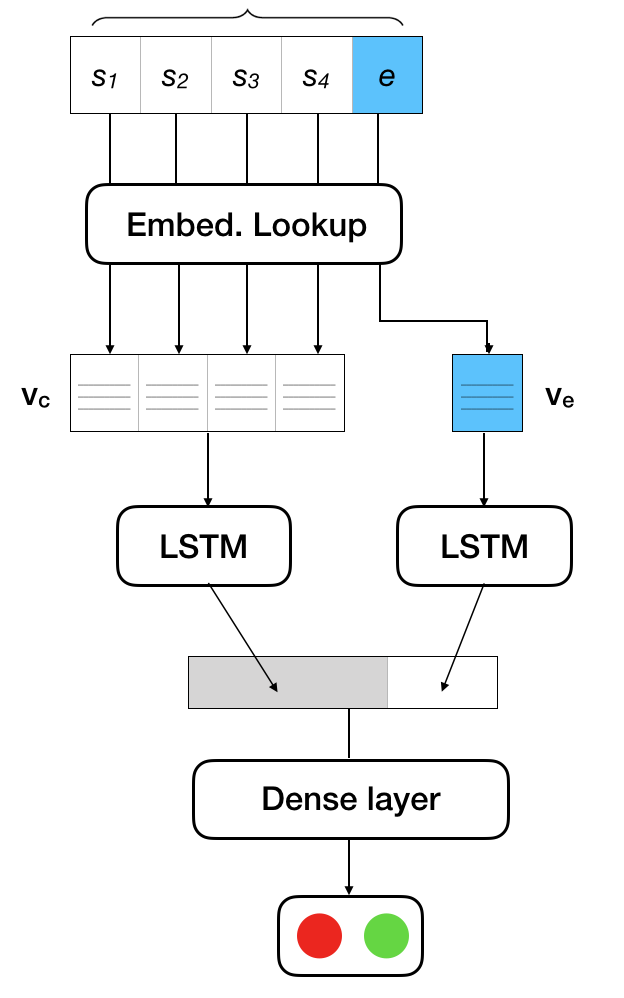
\includegraphics[width=0.5 \linewidth]{fig/ourmodel.png}
  \caption{Our classifier}
  \label{Figure:model}
\end{figure}

\subsection{Wrong ending generation}

\subsubsection{Shuffling} According past publications\cite{top4}, permuting the correct endings of the training stories produce reasonable wrong endings. In our implementation we make sure to use a derangement, i.e. a permutation where no element stays in place. Otherwise we correct endings could appear as negative samples.

\subsubsection{Simple antonyms and negation}

Shuffeling obviously changes the main character and main point of the story. Therefore, we find it sensible to generate endings that are wrong but still preserve the context. Negation of the fifth sentence seemed a promising way to achieve that end. i.e. The resulting sentence would be contain at least one of the charecters of the story. The resulting sentence would still be generally realisitic, except that it would not create a meaningful story as an continuation of the previous four sentences. 

As a first approach we use a few handselected rules. The rules consist of pairs like good/bad and did/didn't. For each pair we replace occurences of the first element with the second element and vice versa. One caveat of this approach is the following scenario: if one elements of the pair occurs much more often then the other, the rare word would appear unreasonably often the wrong endings. For this reason we make sure that the ratio between the two elements of the pairs is the same in the correct and in the wrong endings.


\subsubsection{Wordnet Antonyms}

Negation can be challenging for complex sentence structures because we would have to decide which part of the sentence to negate. For example, for the sentence: "
Kelly quickly went home." There are at least two possibilities of negation: "Kelly slowly went home" or "Kelly did not go home quickly". If we do not keep track the number of negations in the sentence, the result would be wrong: "Kelly did not slowly go home", which is not the negation of the original sentence. Hence, our approach, as shown in Figure \ref{Figure:wrong}, was to first negate the adjectives and adverbs, and in their absence, negate the verbs.

\begin{figure}
  \centering
  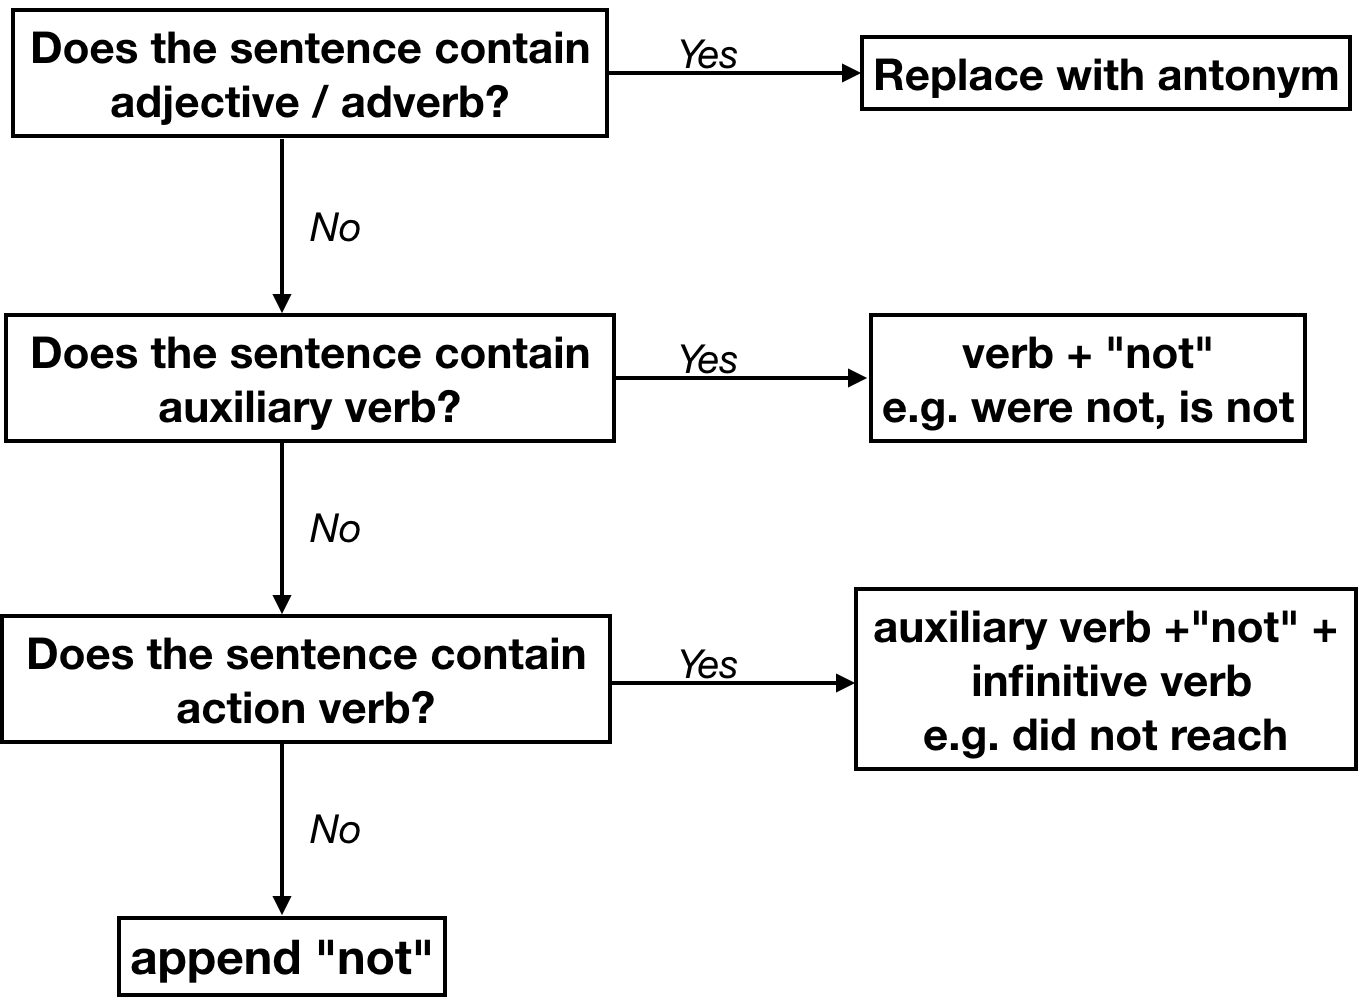
\includegraphics[width=0.7 \linewidth]{fig/wrong.png}
  \caption{Our approach to generate wrong endings}
  \label{Figure:wrong}
\end{figure}


A few examples of our successful sentence generations are shown in Table \ref{Tab:works}

\begin{table}[h]\footnotesize
  \centering

  \begin{tabular}{ p{6cm} p{3cm} p{3cm} }
    \toprule
    Context & Right Ending & Wrong Ending \\
    \midrule
    The family was tired of not hearing when someone knocked on their door. They installed a doorbell on their front door. It would ring a pleasant tune when someone came to see them. They never missed houseguests anymore.  & The family wished they'd gotten the doorbell earlier! & The family wished they'd gotten the doorbell late! \\
    \hline
    Tim was hiking up a mountain with friends. He wasn't paying attention and lost his footing. Tim tumbled down down for a few yards. He was severely hurt. & Tim's friends had to call for help and carry him. & Tim 's friends did not have to call for help and carry him . \\
    \hline
    Laura found a jar of candy in her mom's kitchen. Laura ate all of the candy. She got really sick. Laura's mom discovered why Laura was sick. & Her mom felt bad for her so she didn't punish her for eating it all. & Her mom felt good for her so she didn't punish her for eating it all.\\
    \bottomrule
  \end{tabular}
  \label{Tab:works}
  \caption{Generated wrong endings that works}
\end{table}

\subsubsection{Limitations}
There are two main limitations of our model to generate wrong endings. First, is that our antonym replacement may not be sensible at times \citep{wordnet}. Table \ref{Tab:strange} shows a few examples of sentences are grammatically wrong or not sensible.

\begin{table}[h]\footnotesize
  \centering
  \begin{tabular}{ p{6cm} p{3cm} p{3cm} }
    \toprule
    Context & Right Ending & Wrong Ending \\
    \midrule
    Gina's brother Jay had been out of the house. Now he was back. He'd fought their father. Their dad was a foot taller and 50 pounds bigger. & Gina no longer felt safe with him around. & Gina yes longer felt safe with him around.\\
    \hline
    Matthew grew up with a dad that pushed him in sports.,He thought he would grow up to be an athlete. Once he grew up he realized he wanted to do other things. His dad was very angry. & Their relationship got bad and they no longer talked. & Their relationship got good and they no longer talked. \\
  \bottomrule

  \end{tabular}
  \label{Tab:strange}
  \caption{Generated wrong endings that are not sensible. In the first story, the phrase "yes longer" does not exists in English. In the second story, the sentence is connected by "and" but negation was only applied once.}
\end{table}

Second is that our generated wrong endings may have high occurance of the word "not" as our model was designed to insert "not" in the absence of antonyms. This would affect our classifier performance negatively.

\subsection{Generating wrong endings with a seq2seq model}
We constructed a simple seq2seq model following \cite{tfseq2seq}. The sequence to sequence model consists of two RNNs: an encoder, which reads the input sequence to infer semantics, and a decoder, which generates an output sequence respectively.

We trained the model on 80\% of the validation set. The input sequence is the concatenation of the first four sentences of each story, while the ground truth output sequence is the wrong ending to the story.

In order to be able to train on such a small dataset, pre-training on the training set was performed. This gives the seq2seq model a better understanding of the underlying language.

Because this method uses a portion of the validation set, one could think of instead directly training the classifier on the validation set. 
While a classifier trained directly on the validation set would require an increase in labelled data to improve its performance, our approach can simply generate more wrong endings for potentially unlimited amounts of only semi-labelled data. This is a great advantage, as stories with their right ending are typically more readily available that stories with a corresponding wrong ending.

As can be seen in the results section the generation with the seq2seq model outperforms the other generation methods.

\subsubsection{Limitations}
The sequence to sequence model is currently very simple, restricting its learning capabilities. This means that there is ample room for improvement in this method.


\section{Training}
For the training, the model just learns to predict whether a ending is consistent or not. It doesn't directly learn to decide between two possible endings. We use the validation set in order to stop training before overfitting too much.

\section{Experiments}
For all experiments we use the same classifier, but different wrong endings. To evaluate the quality of our classifier, we do a experiment where we use 80\% of the validation set to train our classifier, and the remaining 20\% as validation set.

\subsection{Results}
\begin{table}[h]
  \centering
  \begin{tabular}{ c c c}
    \toprule
    Approach & Validation & Test \\
    \midrule
    Shuffle & 50.3\% & 50.7\%\\
    Simple Antonyms & 54.4\% & 49.5\%\\
    Wordnet Antonyms & 56.4 & 55.6\\
    Seq2Seq & 63.1 & 59.7\\
    Wordnet \& Seq2Seq & 59.0 & 58.2\\
    All generated & 56.9 & 56.0\\
    Dev set \& Seq2Seq & 69.3 & 66.8\\
    Dev set & 73.3 & 68.0\\

    \bottomrule
    \\
  \end{tabular}
  \label{Tab:results}
  \caption{System accuracies on the Story Cloze datasets. }
\end{table}

\subsection{Final Model for Predictions}

As a final model we use the classifier trained on the seq2seq generated wrong endings and 80\% of the validation set. With this model we produced our submission for the nlu18-testset.

\section{Conclusion}

We showed that sophisticated generation of wrong endings can help train a binary classifier in a meaningful way. Additionaly we propose a seq2seq model which can learn to generate wrong from a very limited fully labeled dataset. The potential of the seq2seq model has been shown, but a more complex model could probably reach a much higher accuracy.

\bibliographystyle{unsrt}
\bibliography{resources.bib}

\end{document}
